\kmuttchapter{THEORETICAL BACKGROUND}
    The first realization of Dirac material started in 1947 when P.R. Wallace proposed the band structure of graphite, or particularly graphene, using the tight binding method.
    At that time, the structure of few layer graphite (later called graphene) was not that popular, since the 2-dimensional crystal was thought to be unstable in normal condition.
    Until 2004, when Andre Geim and Konstantin Novoselov successfully extracted single-atom-thick crystallites graphene from bulk graphite \cite{Zhang2004}.
    This discovery changed how people think about the stability of 2-dimensional crystal structures and their popularity increased accordingly.
    It was pointed out that the electron in these material exhibits massless Dirac particles rather than the usual Schrödinger Hamiltonian \cite{CastroNeto2009}.
    This class of materials are called "Dirac materials".
    The massless relativistic imitation of electron in Dirac materials leads to very high conductivity that is advantageous to high speed nanoelectronic application.
    %Dirac materials are the class of material that posses linear dispersion relation where the conduction and valence bands meet at a single point, called a Dirac point, forming a cone-shaped without energy gap. 
    %Electrons in Dirac material mimic relativistic massless fermion and governed by Dirac equation.

\section{The electronic structure of Dirac materials}
     Tight binding method is commonly used to calculate the band structure of crystals.
     Graphene, for example, has a single layer of carbon atoms forming a perfect 2-dimensional honeycomb structure.
     three of four valence electrons of each carbon atoms form $sp^2$ hybridized orbital and covalently bonded with neighboring carbon atom.
     There is one electron left in $2p_z$ orbital, which is weakly bonded by the Van-der-Waales forces of carbon atom.
     Hence, these electrons are free to move or hop to other carbon atoms with little enough energy.\\
    \begin{figure}[H]
        \centering
        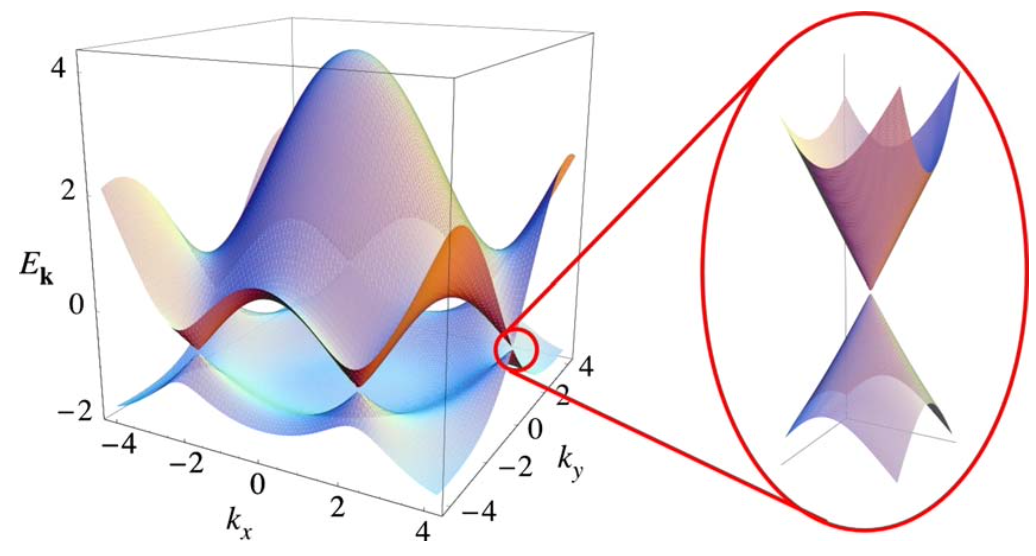
\includegraphics[width = 0.8\linewidth]{fig/Chap 2/band structure of graphene.png}
        \caption{The energy dispersion of graphene. 
                    Left: the full band structure and right: the energy band close to one of the Dirac point.}
        \label{2fig:band structure of graphene}
    \end{figure}
     The tight binding Hamiltonian for electron that can hop to both nearest-neighbor and next-nearest-neighbor atoms is given by
     \begin{equation} \label{2eq:tight binding Hamiltonian}
         \begin{aligned}
             H = &-t \sum_{\braket{\braket{i,j}},\sigma} (a_{\sigma, i}^{\dagger} b_{\sigma,i}^{\dagger}+ \mathrm{H.c.})\\
                    &-t' \sum_{\braket{\braket{i,j}},\sigma} (a_{\sigma, i}^{\dagger} a_{\sigma,i}^{\dagger}+ b_{\sigma, i}^{\dagger} b_{\sigma,i}^{\dagger} + \mathrm{H.c.}),\\
         \end{aligned}
     \end{equation}
     where $t \approx 2.8$ meV is the nearest-neighbor hopping energy of electron, and $t'$ is the next-nearest-neighbor hopping energy.
     $a_{\sigma, i}^{\dagger}$ and $b_{b,i}^{\dagger}$ are creation and annihilation operator, respectively.
     The eigenenergies of Hamiltonian above can be written as
     \begin{equation} \label{2eq:dispersion relation graphene}
        \begin{aligned}
            E_F &= \pm t\sqrt{(3+f(\boldsymbol{k} ))} - t' f(\boldsymbol{k}),\\
            f({\boldsymbol{k}}) &= 2 \cos{(\sqrt{3} k_y a)}+ 4 \cos{\left(\frac{\sqrt{3}}{2} k_y a\right)} \cos{\left(\frac{3}{2} k_x a\right)},\\
        \end{aligned}
     \end{equation}
    where positive and negative sign correspond to the conduction and valence band.
    Fig. \ref{2fig:band structure of graphene} show the full band structure of graphene with nonzero $t$ and $t'$.
    Unlike parabolic dispersion relation of conventional semiconductors, the band structure of graphene close to one of the Dirac points is linear and gapless.
    This linear relation can be obtained analytically by applying the Taylor expansion to Eq. \ref{2eq:dispersion relation graphene} about $q = 0$, 
    where $q = k-K$ is relative wavevector measured from Dirac point
    \begin{equation} \label{2eq:approx energy dispersion}
        E_{\pm}(\boldsymbol{q})\approx \pm v_F |\boldsymbol{q}|        
    \end{equation}
    where $v_F = 3ta/2 \approx 10^6\ \mathrm{m/s}$  is Fermi velocity. 
    The linear relation between energy and wavevector of electron in the low-energy limit indicate that the electron in graphene can be described by Dirac equation.
    In other word, electron in graphene or Dirac material in general, mimics massless relativistic particles.
\section{The classification of Dirac cone materials} \label{2sec: Dirac cone class}
    Dirac cones can be categorized according to the geometry of their Fermi surface.
    The conventional Dirac cone, like those found in graphene, has rotational symmetry about the momentum space. 
    Their Fermi surface is closed and point-like at the band crossing, where the density of states vanishes as shown in Fig. \ref{2fig:type1}.
    However, they are not the only type of Dirac cone that can be found in Dirac materials.
    The general Dirac-like Hamiltonian of two dimensional system is given by
    \begin{equation} \label{2eq:Hamiltonian in dirac cone class}
        H(q) = (w_{x}q_x+w_{y}q_y)\sigma_0 + v_x q_x \sigma_x + v_y q_y \sigma_y,
    \end{equation}
    where $q_{x,y}$ is the wave vector, $v_{x}$ and $v_{y}$ are Fermi velocity in the x- and y-direction, respectively. 
    $w_{x}$ and $w_{y}$ represent the tilted velocities, $\sigma_x$ and $\sigma_y$ are Pauli matrices.
    \begin{figure}[H]
        \centering
        \begin{subfigure}[b]{0.2\linewidth}
            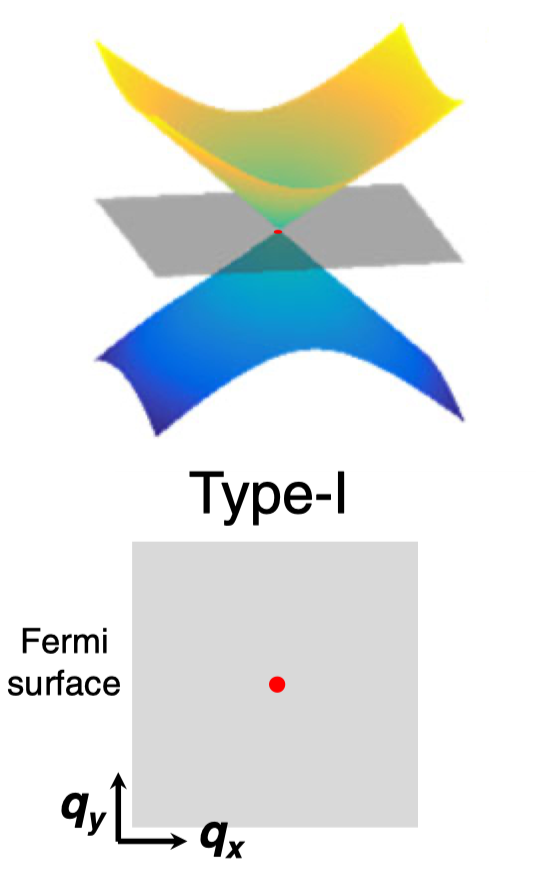
\includegraphics[width = \linewidth]{fig/Chap 2/Type I .png}
            \caption{}
            \label{2fig:type1}
        \end{subfigure}
        \begin{subfigure}[b]{0.2\linewidth}
            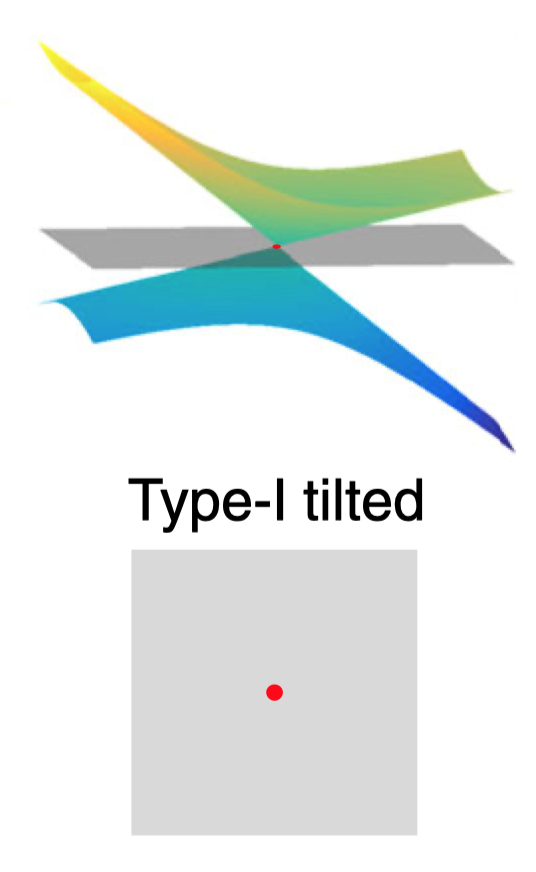
\includegraphics[width = \linewidth]{fig/Chap 2/Type I tilted.png}
            \caption{}
            \label{2fig:type1 tilted}
        \end{subfigure}
        \begin{subfigure}[b]{0.2\linewidth}
            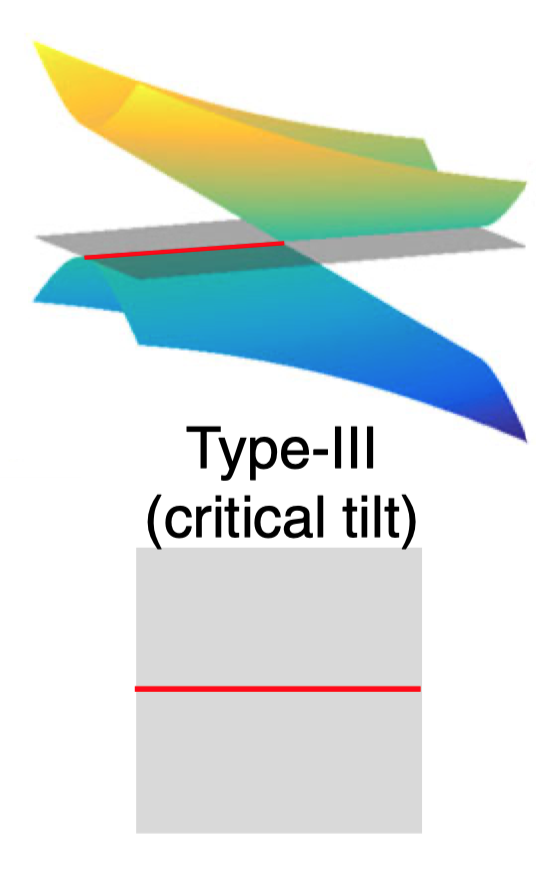
\includegraphics[width = \linewidth]{fig/Chap 2/Type III.png}
            \caption{}
            \label{2fig:type3}
        \end{subfigure}
        \begin{subfigure}[b]{0.2\linewidth}
            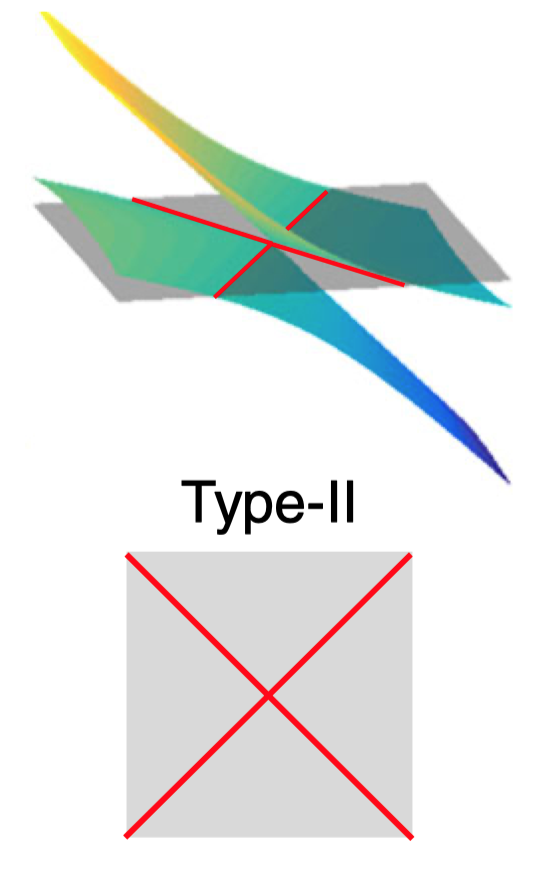
\includegraphics[width = \linewidth]{fig/Chap 2/Type II.png}
            \caption{}
            \label{2fig:type2}
        \end{subfigure}
    \caption{The types of Dirac cone and their corresponding Fermi surface with the zero-energy plane(grey). 
                (a) Type-I Dirac cone characterized by the isotropy of wavevector $k$ and a point-like Fermi surface.
                (b) Type-I tilted Dirac cone, which also has point-like Fermi surface but the wavevector $k$ is anisotropic.
                (c) Type-III Dirac cone with the straight line Fermi surface.
                (d) Type-II Dirac cone.}
    \label{2fig:Dirac cone type}
    \end{figure}
    The eigenenergies of this Hamiltonian can be found as
    \begin{equation} \label{2eq:eigenenergies}
        E_{\pm}(q) w_{x}q_x + w_{y}q_y \pm \sqrt{(v_x q_x)^2 + (v_y q_y)^2}.
    \end{equation}
    If both coefficients $w_{x}$ and $w_{y}$ are zero, the Dirac cone is type-I.
    If $w_{x}$ or $w_{y}$ is nonzero, then the Dirac cone is tilted as shown in Fig. \ref{2fig:type1 tilted}.
    When the tilted parameter
    \begin{equation} \label{2eq:tilted parameter}
        w_0 = \sqrt{\left(\frac{w_x}{v_x}\right)^2 + \left(\frac{w_y}{v_y}\right)^2},
    \end{equation}
    is larger than 1, the Dirac cone is over-tilted and type-II Dirac point is formed.
    The Fermi surface of this type is two crossing lines, and the density of states become finite.
    When the tilted parameter $w_0 = 1$, the Dirac cone situate between type-I tilted and type-II Dirac cones.
    Due to their distinct Fermi surface, the Dirac cone of this kind has been named a type-III Dirac cone.

\section{Borophene: A tilted anisotropic Dirac cone material}
    Graphene was the first one of its kind that successfully synthesized with high stability.
    This material class has been intensively studied due to their superiorly-high surface-volume ratio and novel electronic properties compared with bulk counterparts, one of which is two-dimensional (2D) structure of borons.
    Boron compounds belong to the polyhedral class, which not only results in a large variability of boron compound structure, but also prevents the formation of flat covalent B-B bonding similar to graphene as shown in Fig. \ref{2fig:borophene atomic structure}.
    Despite the potential application of boron-based 2D structure, this material faced a stability problem and its surface is chemically degraded in ambient conditions.
    This stability problem may be solved by the introduction of intrinsic defects \cite{Liu2013}.
    One of the most stable predicted structures of 2D phase of borons is $8-Pmmn$ borophene.
    Their novel electronic properties were revealed by first-principles calculations, which predicted to be semimetallic with anisotropic and tilted Dirac cones \cite{Lopez-Bezanilla2016,Zhou2014}.
    
    \begin{figure}[H]
        \centering
        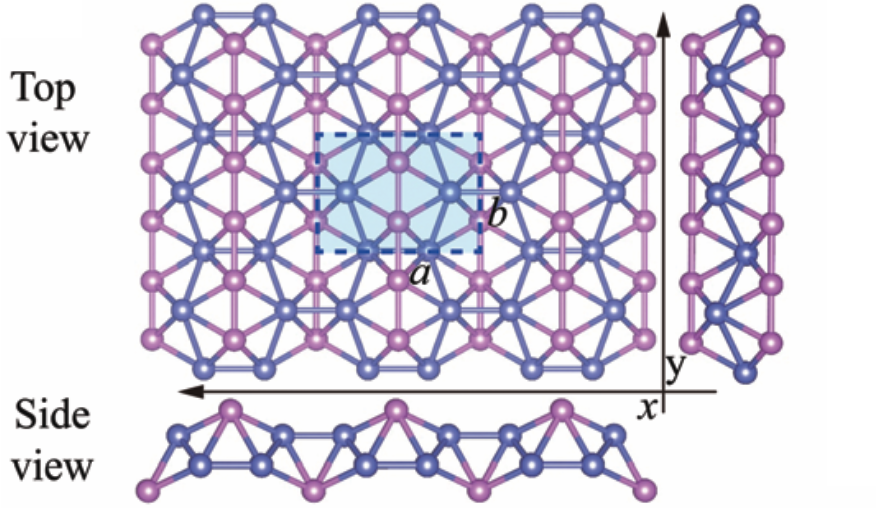
\includegraphics[width = 0.6\linewidth]{fig/Chap 2/borophene atomic structure.png}
        \caption{Atomic structure of $8-Pmmn$ borophene. The two different colors distinguish the two types of nonequivalent B atoms.}
        \label{2fig:borophene atomic structure}
    \end{figure}
    
    Recently, Atomically thin layers borophene has been successfully grown on Ag(111) substrate using a solid boron atomic source under ultrahigh-vacuum conditions \cite{Mannix2015a}.
    This experimental study was extended to the work on synthesis of borophene-graphene heterostructures \cite{Liu2019}.
    They have successfully integrated the borophene into 2D heterostructures with graphene (Fig. \ref{2fig:borophene graphene hetero}).
    Despite the mismatch of crystallographic lattices between borophene and graphene, the rich bonding configurations of boron achieved nearly atomically sharp lateral heterostructures.
    Unfortunately, the experimental realization of transport properties through these heterostructures have not yet been demonstrated.
    Which leaves plenty of room for improvement by the theoretical studies.
    
    \begin{figure}[H]
        \centering
        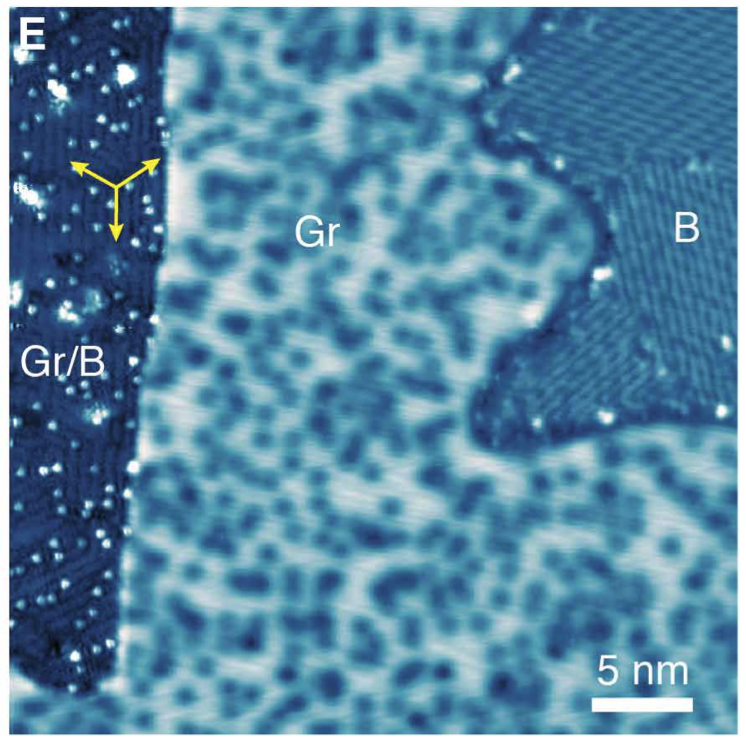
\includegraphics[width = 0.4\linewidth]{fig/Chap 2/borophene graphene.png}
        \caption{STM topography image of lateral and vertical heterostructures of borophene and graphene.}
        \label{2fig:borophene graphene hetero}
    \end{figure}
    


\section{Klein tunneling effect in graphene} \label{2sec:klein effect}
    Klein tunneling refers to a relativistic particles penetrate through the potential barrier without backscattering.
    These properties was once unique to the high-energy particles, where it can only be observed in the system with high-voltage-driven.
    In 2006, this effect is predicted to occur in low-energy system of graphene \cite{Katsnelson2006a}.
    This is because the electron in graphene mimics the relativistic massless Dirac particle and obey massless Dirac equation
    \begin{align} \label{2eq:Hamiltonian}
        \hat{H} = -i\hbar v_F \sigma \nabla 
    \end{align}
    where $v_F \approx 10^6 \mathrm{ms^{-1}}$ is Fermi velocity, $\sigma = (\sigma_x, \sigma_y)$ is Pauli matrix. 
    \begin{figure}[H]
        \centering
        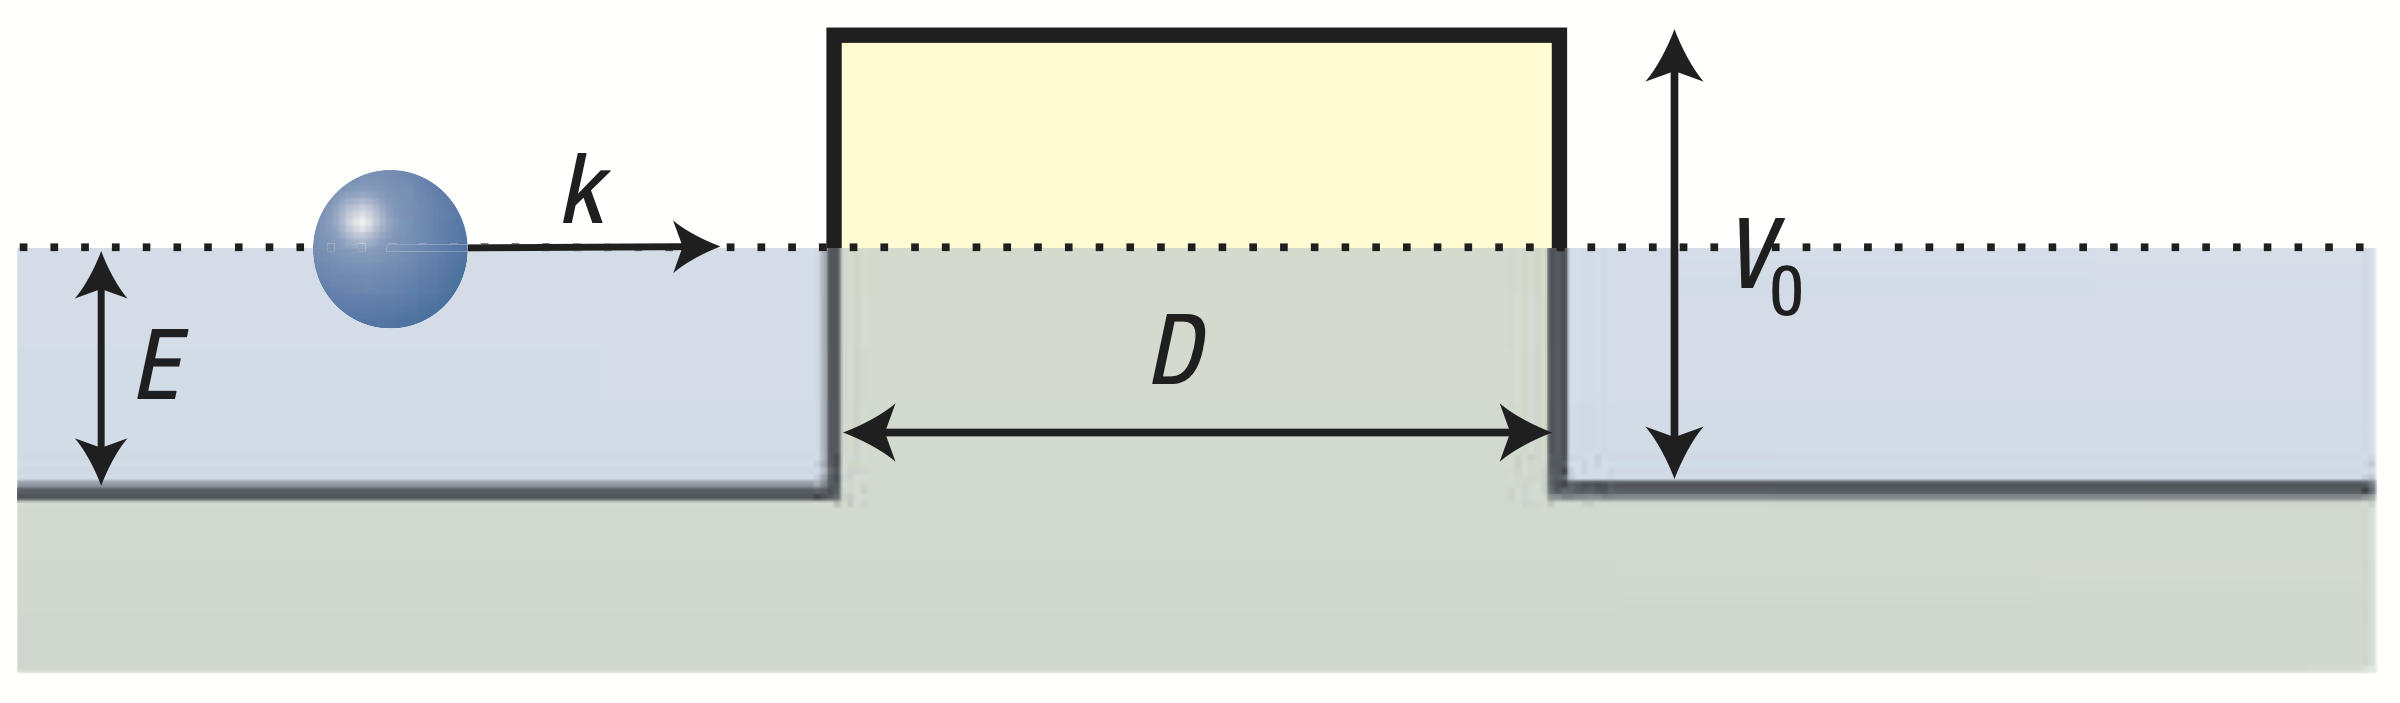
\includegraphics[width=0.7\linewidth]{fig/Chap 2/electron propagation.png}
        \caption{Schematic diagram of electron propagation through the potential barrier of height $V_0$ and width $D$.}
        \label{2fig:electron propagation}
    \end{figure}
    The electron propagation can be modeled as in Fig. \ref{2fig:electron propagation}, consisting of three transport region where the Fermi energy of electron is below the potential barrier.
    By solving Eq. \ref{2eq:Hamiltonian}, the wave function of each region can be expressed as follows
    \begin{equation} \label{2eq:wave function}
        \begin{aligned}
            \psi_1 &= \begin{cases} (e^{ik_x x}+re^{-ik_x x})e^{ik_y y}, &x<0,\\
                (ae^{i q_x x}+be^{-i q_x x})e^{ik_y y},  &0<x<D,\\
                te^{ik_x x + ik_y y},  &x>D,
                \end{cases}\\
            \psi_2 &= \begin{cases} s(e^{ik_x x+i \phi}-re^{-ik_x x-i \phi})e^{ik_y y},  &x<0,\\
                s^\prime(ae^{i q_x x+ i \theta}-be^{-i q_x x- i \theta})e^{ik_y y}, &0<x<D,\\
                ste^{ik_x x + ik_y y+ i \phi}, &x>D,
                \end{cases}
        \end{aligned}
    \end{equation}
    where $k_x = k \cos{\phi}$ and $k_y = k \sin{\phi}$ are x- and y-component wavevector outside the barrier region, respectively.
    $q_x = \sqrt{(E-V_0)^2/(\hbar v_F)^2-k_y^2}$ is x-component wavevector inside the barrier region. 
    $s = \mathrm{sgn}(E)$ and $s^{\prime} = \mathrm{sgn}(E-V_0)$. 
    Since the wave function of each region has to be continuous at the boundary, we can substitute $x = 0$ and $x = D$ to Eq. \ref{2eq:wave function}, which give
    \begin{equation} \label{2eq:boundary condition}
        \begin{aligned}
            1+r-a-b&=0\\
            s(e^{i\phi}-e^{-i\phi}r)-s\prime (e^{i\theta}a-e^{-i\theta}b)&=0\\
            e^{iDq_x}a+e^{-iDq_x}b-e^{iDk_x}t&=0\\
            s \prime (e^{iDq_x+i\theta}a-e^{-iDq_x-i\theta} b)-se^{iDk_x+i\phi}t&=0\\
        \end{aligned}
    \end{equation}
    where r and t is the reflection and transmission coefficient, respectively. Which can be obtained by solving the system of equations above.
    The reflection coefficient has the following expression
    \begin{align} \label{2eq:reflection coefficient}
        r=2ie^{i\phi}\sin{(q_xD)}\times\frac{\sin{\phi}-ss^{\prime}\sin{\theta}}{ss^{\prime}[e^{-iq_xD}\cos{(\phi+\theta)}+e^{iq_xD}\cos{(\phi-\theta)}]-2i\sin{(q_xD)}}
    \end{align}
    Since $T = |t|^2 = 1-|r|^2$, the transmission probability can be expressed as follow
    \begin{align} \label{2eq:transmission probability}
        T = \frac{\cos^2{\phi}}{1-\cos^2{(q_x D)}\sin^2{\phi}}
    \end{align}
    Fig. \ref{2fig:Klein tunneling} shows the polar plot of Eq. \ref{2eq:transmission probability}. 
    At the incident angle $\phi = 0$, electron tunnels through the barrier with probability of one no matter the height of the potential barrier.
    This is the feature unique to massless Dirac fermion called Klein tunneling.
    \begin{figure}[H]
        \centering
        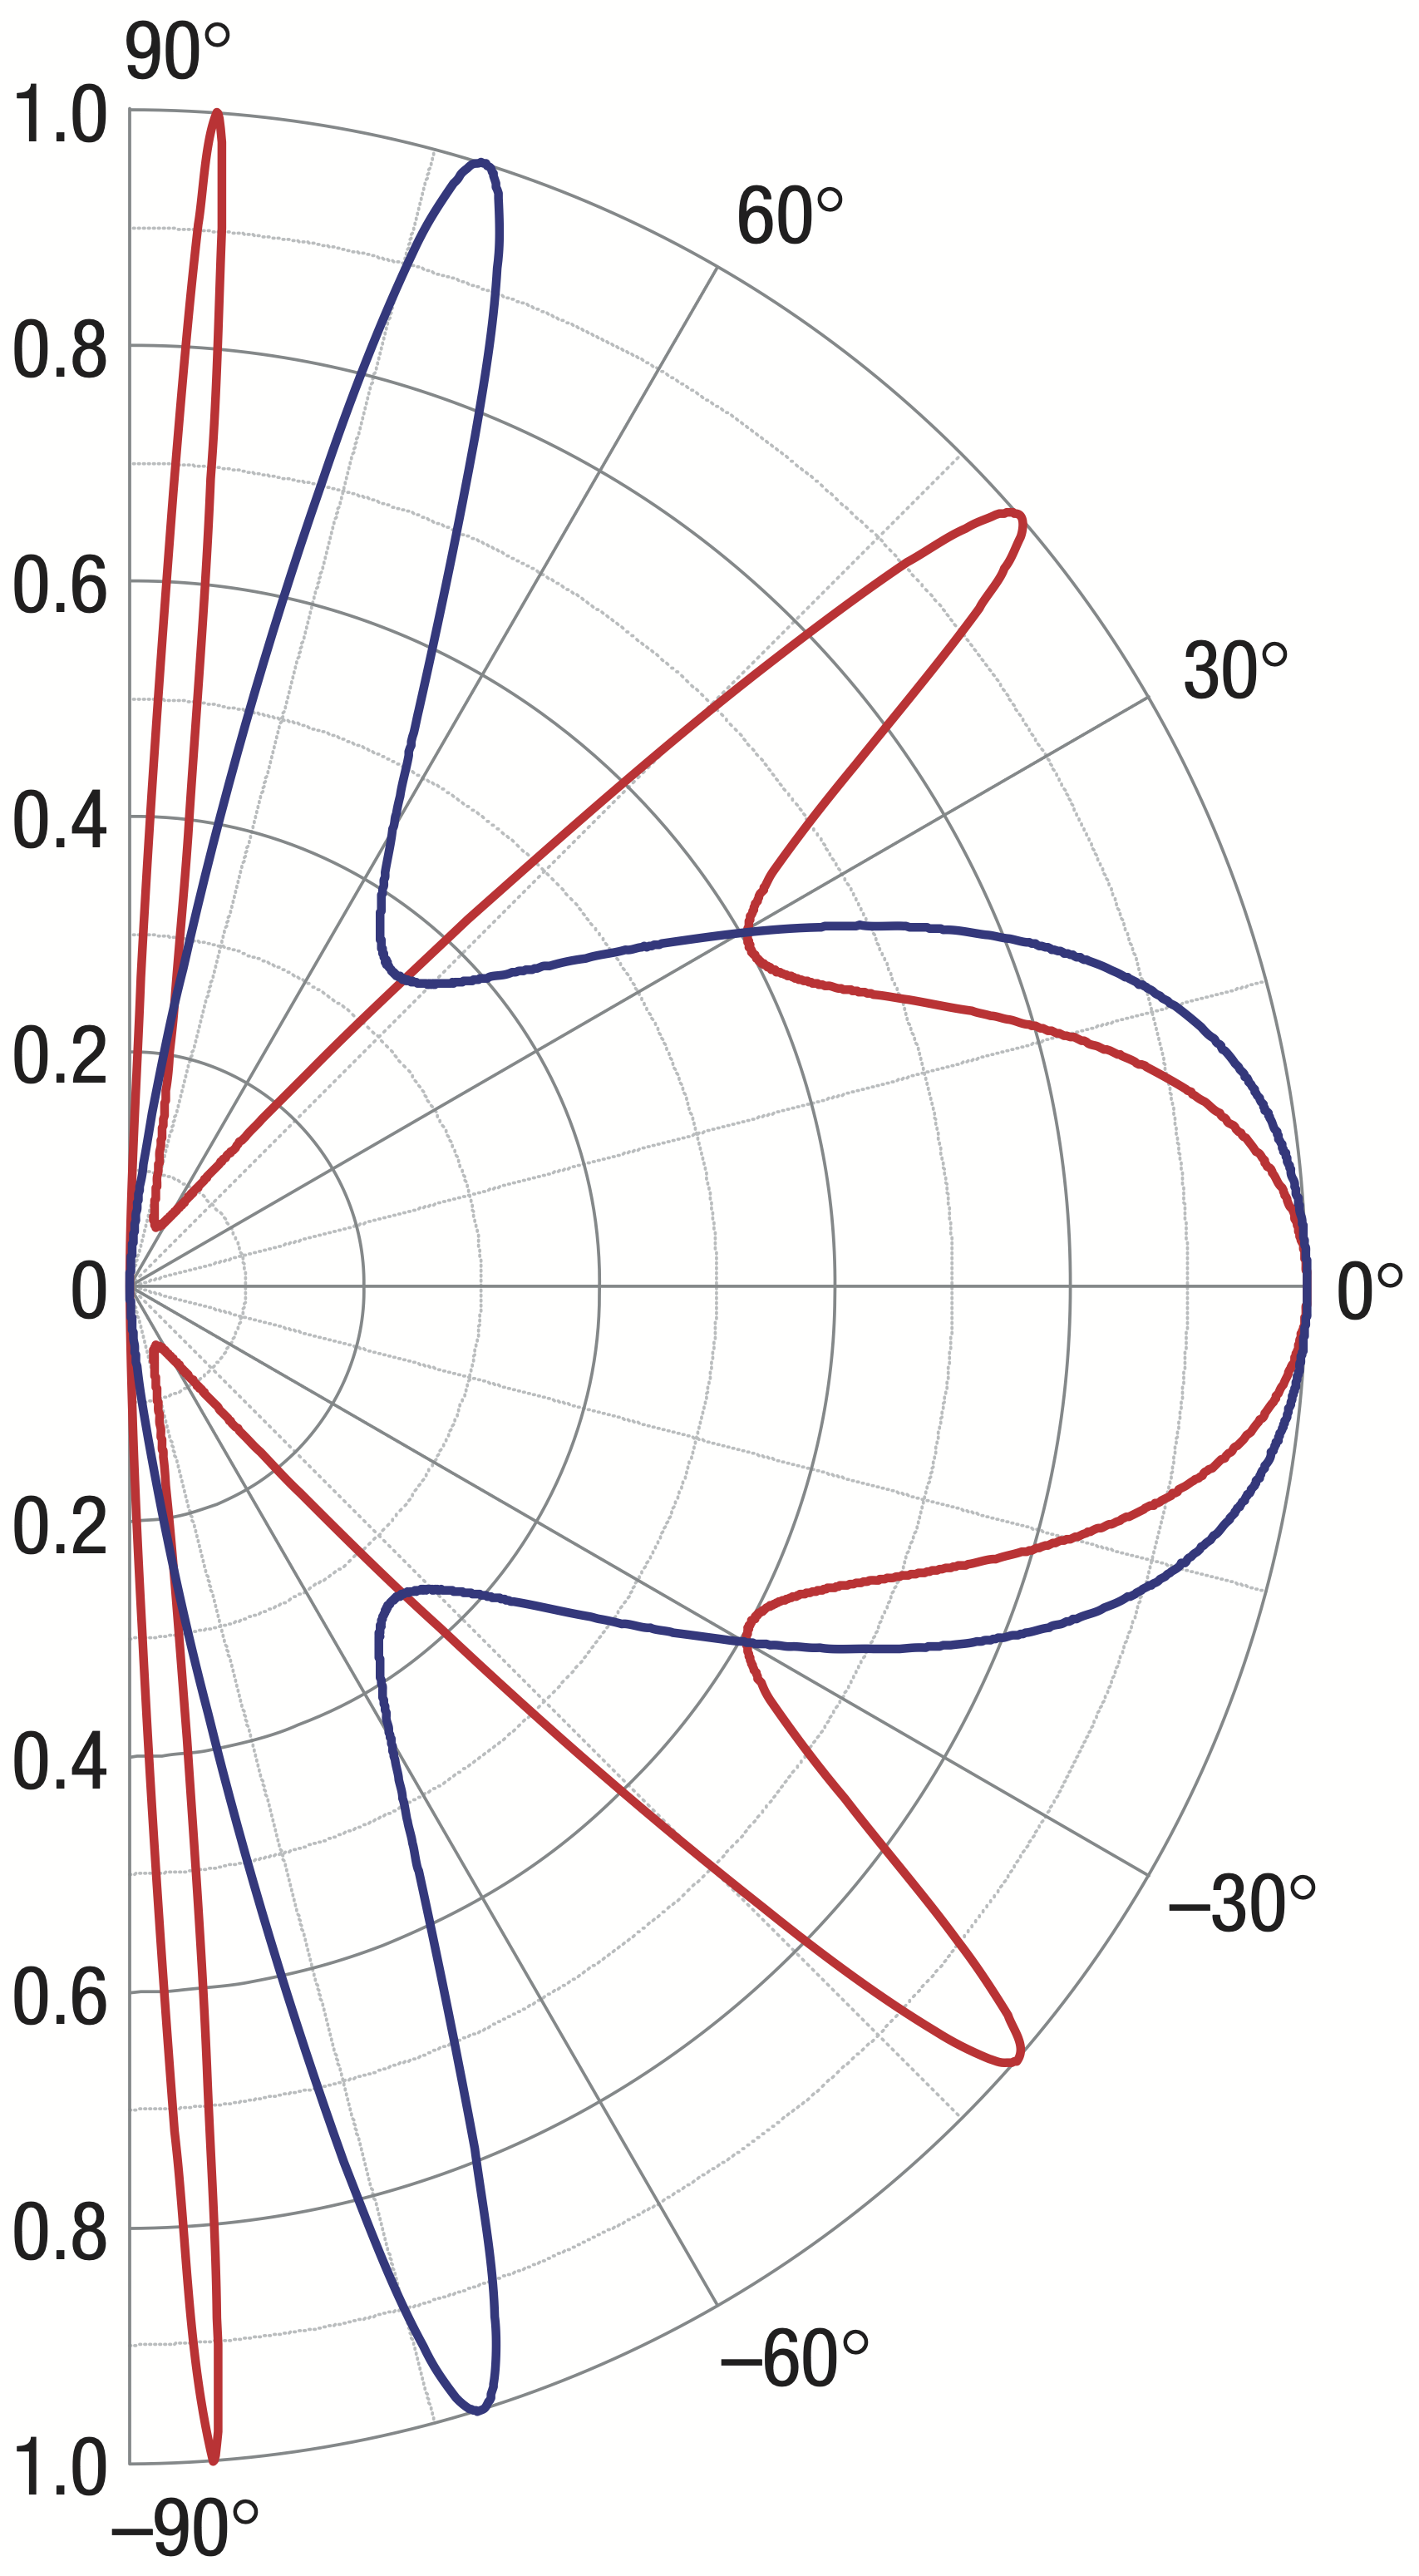
\includegraphics[width = 0.3\linewidth]{fig/Chap 2/klein tunneling.png}
        \caption{The transmission probability as a function of incident angle with different barrier height. 
                    $V_0 = 200$ meV for red curve and $285$ meV for blue curve.}
        \label{2fig:Klein tunneling}
    \end{figure}
    Moreover, Eq. \ref{2eq:transmission probability} also results in perfect transmission at nonzero incident angles, which occurred under the resonance condition $q_x D = \pi N$, $N = 0, \pm 1,...$.
    These perfect tunnelings are similar to Fabry-Perot interference in optics, where the incoming light rays constructively interfere with itself inside the cavity.
    These angle-dependent transmissions were experimentally investigated in graphene heterojunctions \cite{Rahman2015}.
    The setup for measuring the angle-dependent transmission is shown in Fig. \ref{2fig:3 arm device}.
    The measurement is carried out by applying the current bias between arm 1 and the other three arms, where the measurements are reported as the resistance of each arm as shown in Fig. \ref{2fig:r vs v}.
    These resistances  can be measured using standard four-probe technique.
    \begin{figure}[H]
        \centering
        \begin{subfigure}[b]{0.5\linewidth}
            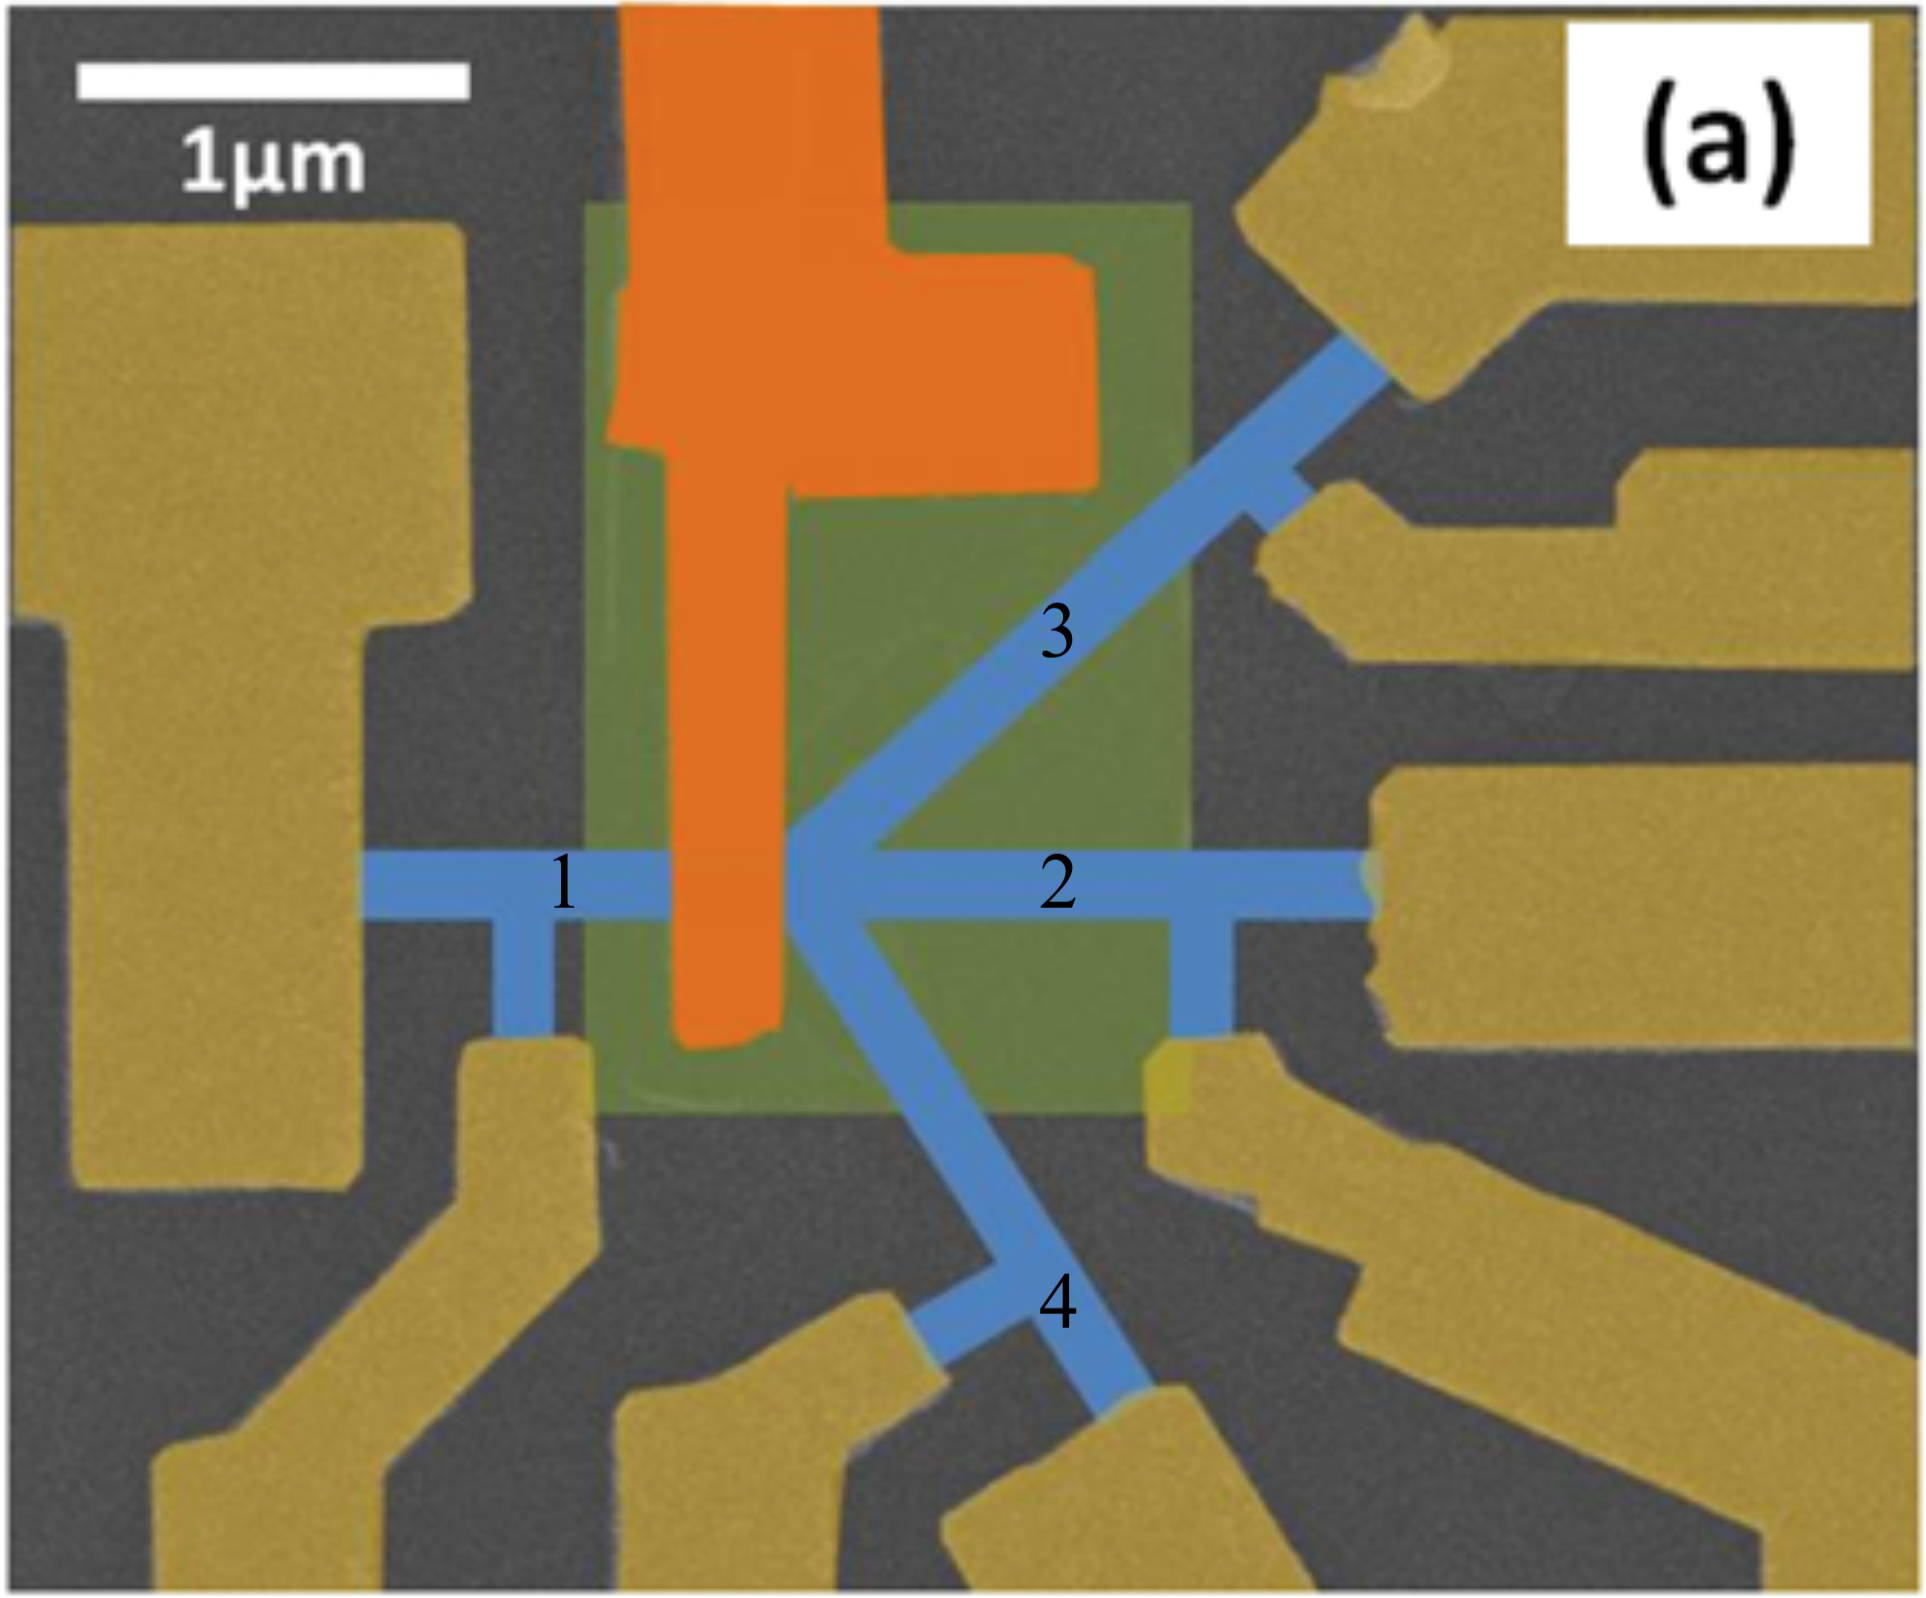
\includegraphics[width = \linewidth]{fig/Chap 2/angle-dependent transmission.png}
            \caption{}
            \label{2fig:3 arm device}
        \end{subfigure}
        \begin{subfigure}[b]{0.35\linewidth}
            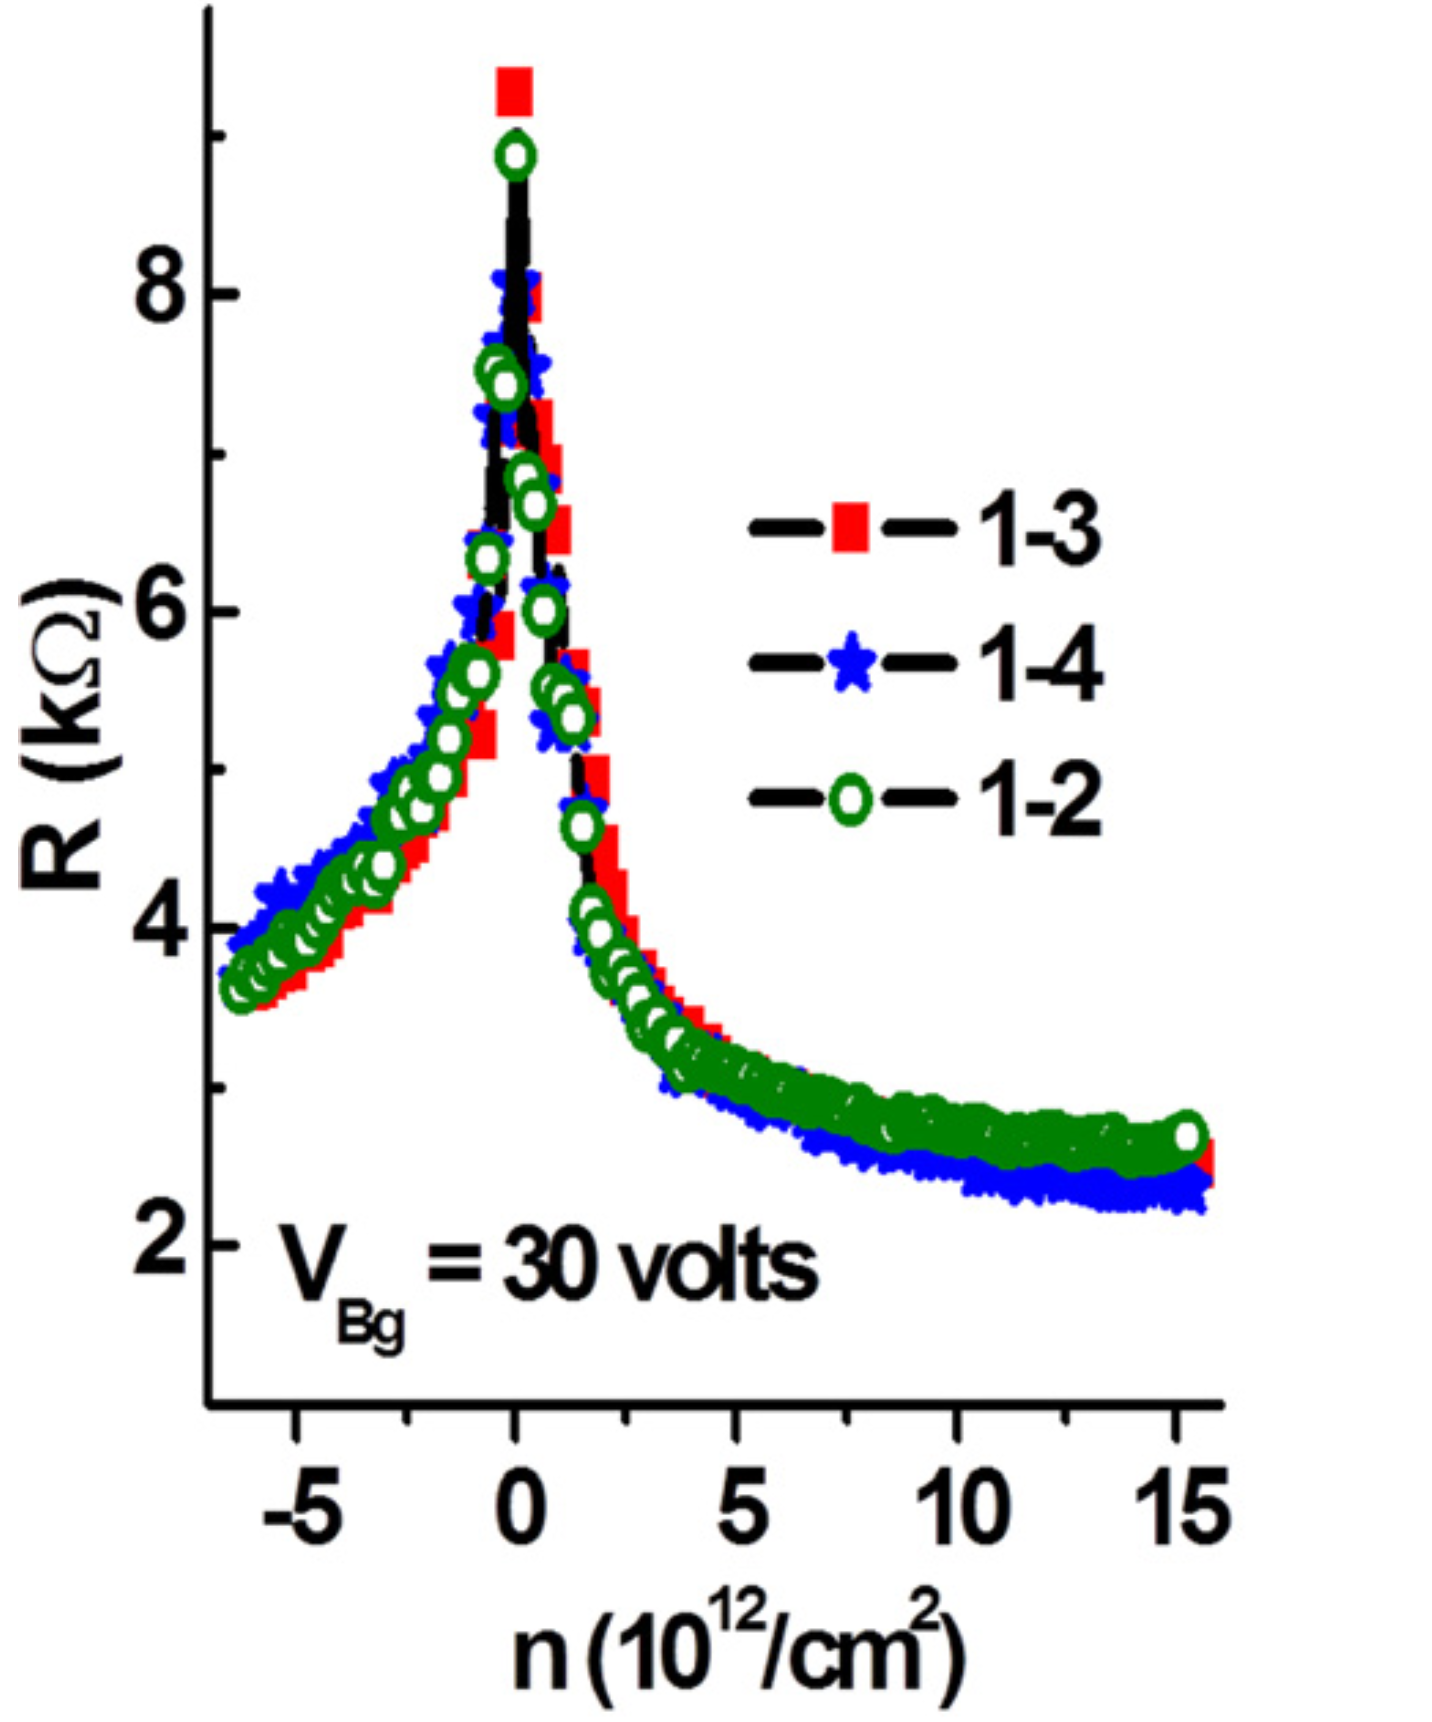
\includegraphics[width = \linewidth]{fig/Chap 2/R vs V.png}
            \caption{}
            \label{2fig:r vs v}
        \end{subfigure}
        \caption{(a) SEM image of single layer graphene device with straight and angles arms(blue). 
                    The angled arms are $45^{\circ}$ with the straight arm. 
                    The bottom and top gate are shown in green and orange, respectively. The leads are shown in yellow.
                    (b) Resistance as a function of carrier density under the application of top gate voltage for arms 2, 3, and 4. 
                    $V_{Bg}$ is bottom gate voltage.}
        \label{2fig:angle dependent transmission}
    \end{figure}
\section{Electronic transport of electron in Weyl semimetals under the influence of magnetic field} \label{2sec:transport in B field}
    %A two-dimensional electron gas in graphene is closely related to light propagation in geometrical optics, where the electron penetrating the potential barrier is analogous to negative refraction through metamaterials.

    In the previous section, we introduced the characteristic transport behavior of electron in graphene such as the leakage of electron current due to the perfect tunneling at normal incident known as Klein tunneling.
    The discovery of graphene has enabled us to observed this uncommon effect in a condensed matter system \cite{Zhang2004}.
    The electron tunneling through the potential barrier has been studied both theoretically and experimentally \cite{Katsnelson2006a,Allain2011,Rahman2015}.
    In this section, we show the transport behavior of electron in 3-dimensional Weyl semimetal with the magnetic barrier.
    \begin{figure}[H]
        \centering
        \begin{subfigure}[b]{0.6\linewidth}
            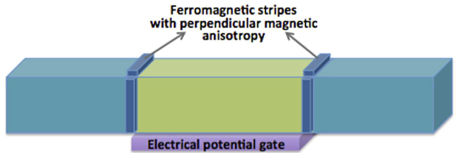
\includegraphics[width = \linewidth]{fig/Chap 2/2weyl structure.png}
            \caption{}
            \label{2fig:weyl structure}
        \end{subfigure}
        \begin{subfigure}[b]{0.6\linewidth}
            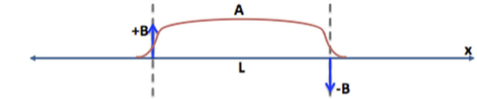
\includegraphics[width = \linewidth]{fig/Chap 2/B field profile.png}
            \caption{}
            \label{2fig:b field profile}
        \end{subfigure}
        \begin{subfigure}[b]{0.6\linewidth}
            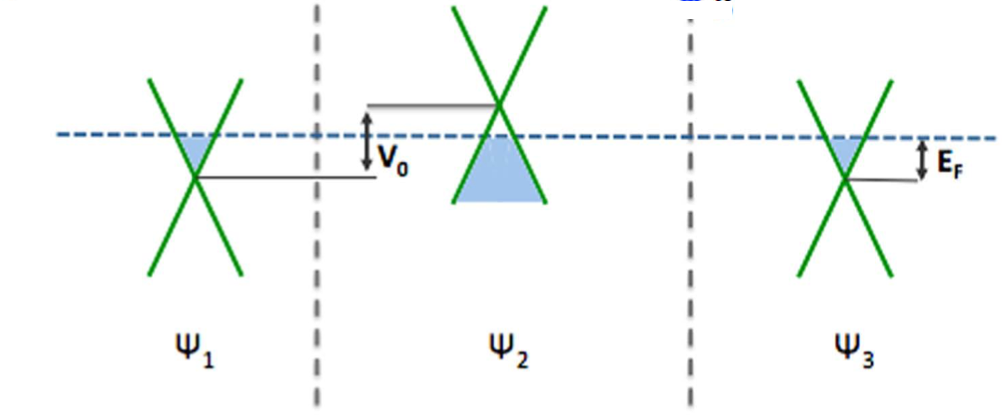
\includegraphics[width = \linewidth]{fig/Chap 2/three weyl cones.png}
            \caption{}
            \label{2fig:3 weyl cones}
        \end{subfigure}
        \caption{The schematic illustration of the single potential barrier Weyl semimetal under the influence of magnetic field 
                    induced by four ferromagnetic stripes on the top and one side surfaces.}
        \label{2fig:weyl npn}
    \end{figure}
    The device structure is shown in Fig. \ref{2fig:weyl structure}, where the delta-function magnetic fields at the barrier interfaces cause following gauge potentials on z- and y- directions
    \begin{equation} \label{2eq:b field profiles}
        \begin{aligned}
            \vec{A}_{B_z} = B_{0(z)}l_B[\Theta(x)-\Theta(x-L)]\hat{y}\\
            \vec{A}_{B_y} = B_{0(y)}l_B[\Theta(x)-\Theta(x-L)]\hat{z}\\
        \end{aligned}
    \end{equation}
    where $l_B =  \sqrt{\frac{\hbar}{|e| B_0}}$. 
    Since the magnetic vector potential has an effect on electron momentum, the Hamiltonian of this system is given by
    \begin{equation} \label{2eq:Hamiltonian with b}
        H = v_F (\sigma . (p + eA) ) +V_0.
    \end{equation}
    where $v_F$ is the Fermi velocity, and $\sigma$ is Pauli matrices. 
    For simplicity, we consider Weyl electrons near one node and neglect the contribution of surface states and intervalley scattering.
    By considering the electron propagation along x-direction, the eigenfunctions of Eq. \ref{2eq:Hamiltonian with b} can be obtained as
    \begin{equation} \label{2eq:eigenfunctions b field}
        \psi_{\pm} \equiv \frac{1}{\sqrt{2}}e^{ikr} 
        \begin{pmatrix}
            1\\
            e^{i \phi} \sec{\gamma}(\pm 1 + \sin{\gamma})\\
        \end{pmatrix} \equiv
        \begin{pmatrix}
            \psi_a\\
            \psi_b^{\pm}
        \end{pmatrix}
    \end{equation}
    The $\psi_a$ component for each regions in Fig. \ref{2fig:3 weyl cones} can be written as
    \begin{equation} \label{2eq:a wavefunctions b field}
        \begin{aligned}
            &\Psi_{1,a}(x) = e^{ik_x x}+ r e^{-i k_x x}, &x<0,\\
            &\Psi_{2,a}(x) = ae^{i q_x x}+ b e^{-i q_x x}, &0<x<L,\\
            &\Psi_{3,a}(x) = te^{ik_x x}, &x>L.\\
        \end{aligned}
    \end{equation}
    The $\psi_b$ component can be found using the relation $\psi_2 = e^{i \phi} \sec{\gamma}(s + \sin{\gamma})\psi_1$, where $s = \pm 1$ depending on the sign of energy $(E_F -V_0)$
    \begin{equation} \label{2eq:b wavefunctions b field}
        \begin{aligned}
            &\Psi_{1,b}(x) = e^{i \phi} \sec{\gamma}(1 + \sin{\gamma})e^{ik_x x}- re^{-i \phi} \sec{\gamma}(1 + \sin{\gamma}) e^{-i k_x x}, &x<0,\\
            &\Psi_{2,b}(x) = ae^{i \theta} \sec{\alpha}(s + \sin{\alpha})e^{i q_x x}- be^{-i \theta} \sec{\alpha}(s + \sin{\alpha}) e^{-i q_x x}, &0<x<L,\\
            &\Psi_{3,b}(x) = te^{i \phi} \sec{\gamma}(1 + \sin{\gamma})e^{ik_x x}, &x>L.\\
        \end{aligned}
    \end{equation}
    The Fermi wavevector is 
    \begin{equation} \label{2eq:fermi wavevector}
        k_F = \sqrt{k_x^2+k_y^2+k_z^2} 
    \end{equation}
    where $k_x = k_F \cos{\gamma}\cos{\phi}$, $k_y = k_F \cos{\gamma} \sin{\phi}$, $k_z = k_F \sin{\gamma}$. 
    The x-component wavevector inside the barrier is 
    \begin{equation} \label{2eq:fermi wavevector in barrier}
        q_x = \sqrt{\left(\frac{E_F-V_0}{\hbar v_F}\right)^2-k_y^2-k_z^2}
    \end{equation}
    The propagating angles inside the barrier can be found by considering the conservation of y- and z-component wavevectors
    \begin{equation}\label{2eq:propagaing angles}
        \begin{aligned}
            \theta = \tan^{-1}\left(\frac{k_y}{q_x}\right)\\
            \alpha = \tan^{-1}\left(\frac{k_z}{q_x} \cos{\theta}\right)\\
        \end{aligned}
    \end{equation}
    
    Since the effect of magnetic vector potential shifts the transverse wavevectors $k_y \rightarrow k_y + \frac{eA_{B_y}}{\hbar}$, $k_z \rightarrow k_z + \frac{eA_{B_z}}{\hbar}$,
    the wavevectors along these directions have to be recalculated with the contribution of magnetic field, which can be written as
    \begin{equation} \label{2eq:transverse k with b field}
        \begin{aligned}
            k_y &= \frac{E_F \cos{\gamma} \sin{\phi}+ \eta v_F \sqrt{|B_{0(y)}|\hbar |e|}}{\hbar v_F},\\
            k_z &= \frac{E_F \sin{\gamma}+ \eta v_F \sqrt{|B_{0(z)}|\hbar |e|}}{\hbar v_F},\\
        \end{aligned}
    \end{equation}
    where $\eta = \pm 1$ depending on the sign of the magnetic field.\\

    First consider the transmission profiles in Fig. \ref{2fig:klein b field} in the case of no applied magnetic field (blue curves).
    When $V_0$ is close to $E_F$, the Fermi level is very close to the Weyl node in the barrier region. 
    Therefore, only the normal incident electron $(\gamma \approx 0$ and $\theta \approx 0)$ or Klein tunneling in particular, can be transmitted perfectly as shown in Fig. \ref{2fig:klein b field 1}.
    When $V_0$ is much greater than $E_F$, we also achieve the Klein tunneling effect but with the additional perfect transmissions.
    These perfect transmissions can be understood by the resonance condition of Fermi wavevector $k_F$ and the barrier length $L$, which can be derived using the relation $q_x L = n \pi$,
    
    \begin{equation}\label{2eq:resonance condition}
        L \sqrt{\left(\frac{E_F-V_0}{\hbar v_F}\right)^2-k_F^2 \sin^2{\gamma}-k_F^2 \cos^2{\gamma} \sin^2{\phi}}= n \pi,
    \end{equation}
    where $n = 0, \pm 1,...$ . When the resonance condition above is satisfied, the angular perfect tunneling occurred as shown in Fig. \ref{2fig:klein b field 2}.
    The number and shape of the perfect transmissions can be intuitively predicted since they are highly dependent on applied voltage and Fermi energy.
    When the magnetic barrier is applied to the system, the transmission profiles become asymmetric, where the direction of the shift depend on the direction of the magnetic barrier.
    The influence of the magnetic field or magnetic vector potential to be specific, is actually shifts the Weyl cone in the transverse direction.
    For this reason, with enough magnetic field strength, The Klein tunneling will be destroyed as the red and brown curve in Fig. \ref{2fig:klein b field 1}. 
    \begin{figure}[H]
        \centering
        \begin{subfigure}[b]{0.4\linewidth}
            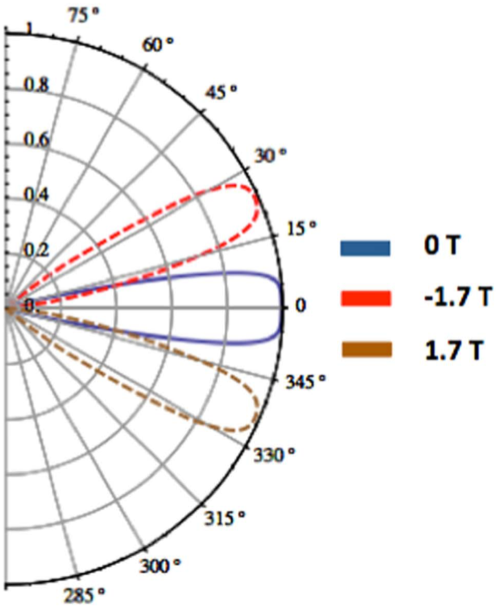
\includegraphics[width = \linewidth]{fig/Chap 2/klein b field 1.png}
            \caption{}
            \label{2fig:klein b field 1}
            \end{subfigure}
            \begin{subfigure}[b]{0.4\linewidth}
                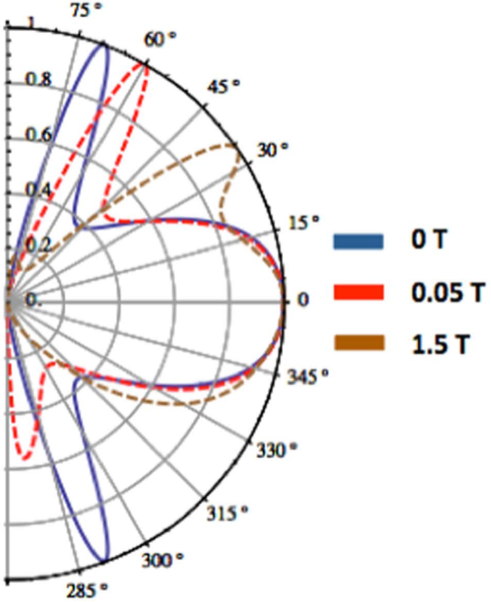
\includegraphics[width = \linewidth]{fig/Chap 2/klein b field 2.png}
                \caption{}
                \label{2fig:klein b field 2}
            \end{subfigure}
        \caption{The polar plot of transmission probabilities in the presence of different strength of applied magnetic barrier, 
                    where the angle between z-axis and xy-plane $\alpha = 0$. 
                    The potential barrier height is (a) 285 meV and (b) 63 meV, where the Fermi energy is 83 meV and barrier length is 100 nm.}
        \label{2fig:klein b field}    
    \end{figure}
\section{Asymmetric tunneling of electron in tilted Weyl cone systems} \label{2sec:asymmetric tunneling}
    The electronic structure of pristine graphene is often symmetric and non-tilted, 
    which indicate that the transmission of electron is symmetric with respect to normal incident angle as shown in section \ref{2sec:klein effect}.
    Unlike the Dirac cone of graphene, in 3-dimensional Weyl semimetals, the Weyl cone around the Weyl point is generally tilted and anisotropic as Weyl points are not located on high-symmetry k-points.
    A tilted Weyl fermion can be described by the low energy Weyl Hamiltonian with asymmetric velocities
    \begin{align}\label{2eq:Hamiltonian titled}
        H = V_0 + \sum_{i} \hbar k_i(\sigma^{i} v_i + w_i) 
    \end{align}
    where $\sigma^i$ are the Pauli matrices, $v_i$ are the velocities in 3 dimensions, and $V_0$ is the potential barrier height.
    $w_i$ is the tilt of Weyl cone in the unit of velocity. The model of interest is shown in Fig. \ref{2fig:weyl transistor} with the potential profile $V_{(x)} = V_0[\Theta(x)-\Theta(x-L)]$.
    By solving the Hamiltonian above, the components of the wave functions are written as
    \begin{align} \label{2eq: wave functions}
        \psi_{\pm} = \frac{1}{\sqrt{2}}e^{i \vec{k}\ \vec{r}}
        \begin{pmatrix}
            1 \\
            e^{i \phi} \sec{\gamma (\pm 1 + \sin{\gamma})}
        \end{pmatrix}= 
        \begin{pmatrix}
            \psi_a \\
            \psi_b^{\pm}
        \end{pmatrix}   
    \end{align}
    The transmission probability can be calculated by matching both components of the wave functions at the interfaces.
    The wave vector outside the potential barrier is expressed as
    \begin{equation}\label{2eq:outside wavevector}
        \begin{aligned} 
            k_x &= k_F \cos{\gamma} \cos{\phi},\\
            k_y &= k_F\cos{\gamma} \sin{\phi},\\
            k_z &= k_F \sin{\gamma}\\
        \end{aligned}
    \end{equation}
    and wave vector inside the potential barrier is
    \begin{align} \label{2eq:inside wavevector}
        q_x = \frac{\sqrt{(E_F-V_0-\hbar k_y w_y)^2 - \hbar^2 v_F^2 (k_y^2 + k_z^2)}}{\hbar v_F}.
    \end{align}
    The angles of electron propagation inside the potential barrier 
    \begin{equation} \label{2eq:angles}
        \begin{aligned}
            \theta &= \arctan{\left(\frac{k_y}{q_x}\right)},\\
            \alpha &= \arctan{\left(\frac{k_z}{q_x} \cos{\theta}\right)}.\\
        \end{aligned}
    \end{equation}
    can be calculated by considering the conservation of the transverse wave vectors $k_y$ and $k_z$ at the barrier interface $x = 0$. 
    \begin{figure}[H] 
        \centering
        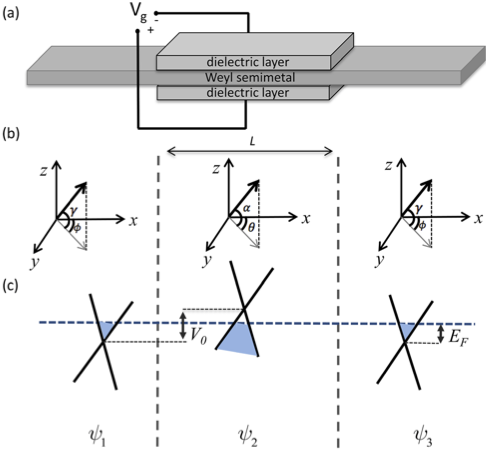
\includegraphics[width = 0.6\linewidth]{fig/Chap 2/2transistor.png}
        \caption{The schematic illustration of a Weyl semimetal under the influence of potential barrier of width $L$ and height $V_0$.}
        \label{2fig:weyl transistor}
    \end{figure}


    In the case of non-tilted Weyl cone system, the transmission probability is symmetric with respect to $\phi = 0$ and $\gamma = 0$ as shown in Fig. \ref{2fig:anomalous1}.
    Which similar to the transmission of electron in graphene except that it is confined to two dimensions, whereas the Weyl semimetal is three dimensions.
    This symmetric transmission becomes asymmetric when the Weyl cone is tilted along one of the transverse directions as shown in Fig. \ref{2fig:anomalous2}.
    In other word, the transmission is shifted to the direction of the tilt. 
    This can be understood by considering the Fermi surfaces in Fig. \ref{2fig:anomalous fermi surface}.
    In the case of $\phi > \phi_{a,b}$, $q_x$ becomes imaginary and the electron is totally reflected.
    The shaded angles show the allowed range where the electron can propagate through the barrier.
    The analytical form of the critical angle of incident electron is found as
    \begin{equation} \label{2eq:phi a}
        \phi_a = \sin^{-1}{\left(- \frac{v_F (V_0 - E_F)}{E_F v_F - V_0 w_y}\right)}
    \end{equation}
    In the previous studies, the asymmetric transmission was only analyzed in the system with step magnetic or strain gauge potential \cite{Pereira2009,Fujita2010,Wu2010}.
    Fig. \ref{2fig:anomalous fermi surface2} shows the Fermi surface under the influence of magnetic step vector potential $A_y = B_0 l_B \Theta (x)\hat{y}$, where $l_B = \sqrt{\frac{\hbar}{|e|B_0}}$, 
    which was shifted by the amount of $k_y = k_y + \delta k_B$.
    In this case, the critical angle of incident electron is found as
    \begin{equation} \label{2eq:phi b}
        \phi_b = \sin^{-1}{\left(-\frac{V_0 - E_F + \eta v_F \sqrt{|B_0 \hbar e|}}{E_F}\right)}
    \end{equation}
    where $\eta = \mathrm{sign}(B_z)$. The equivalent y-component wavevector shifted due to the tilted Weyl cone and potential barrier can be approximately derived by considering the average of shift
    at the maximum and minimum points of $k_y$.
    By equating Eq. \ref{2eq:phi a} and \ref{2eq:phi b}, the delta function pseudo-magnetic field generated by the application of potential barrier and tilted Weyl cone is given by

    %in the case of $w_y \neq 0$, the limit of electron incident angle is 

    %This asymmetric transmission is actually similar to the transmission under the influence of magnetic field.
    %To understand this analytically, consider Eq. \ref{2eq:inside wavevector}, the wave vector inside the barrier region $q_x$
    \begin{align} \label{2eq:pseudo b}
        B \approx \frac{V_0^2 w_y^2}{e \hbar (w_y^2-v_F^2)^2}
    \end{align}
    The transmission under the influence of magnetic vector potential is shown in Fig. \ref{2fig:anomalous6}, where the magnetic field strength is calculated by Eq. \ref{2eq:pseudo b} for $V_0 = 160$ meV and $w_y = 0.1 v_F$.
    The result almost identical to those of the tilted Weyl semimetal without the magnetic barrier (see Fig. \ref{2fig:anomalous2}).
    \begin{figure}[H]
        \centering
        \begin{subfigure}[b]{0.4\linewidth}
            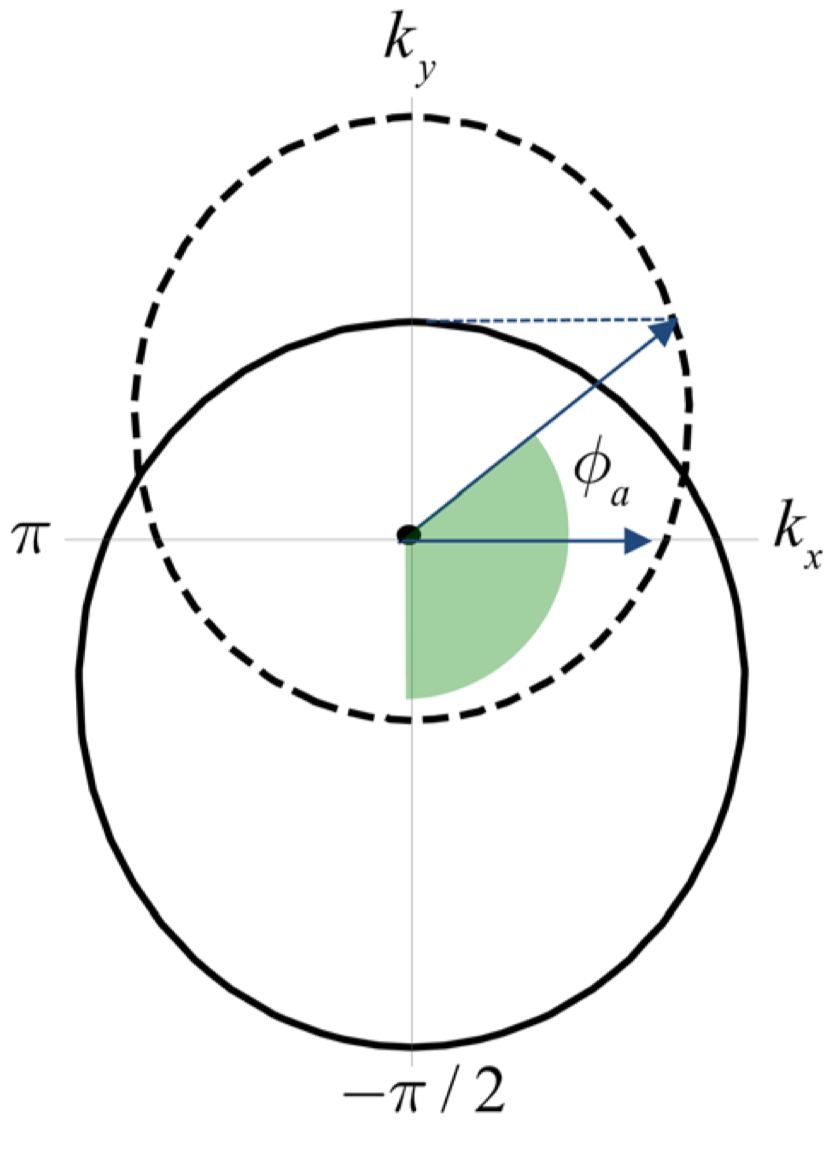
\includegraphics[width = \linewidth]{fig/Chap 2/anomalous fermi surface1.png}
            \caption{}
            \label{2fig:anomalous fermi surface1}
        \end{subfigure}
        \begin{subfigure}[b]{0.4\linewidth}
            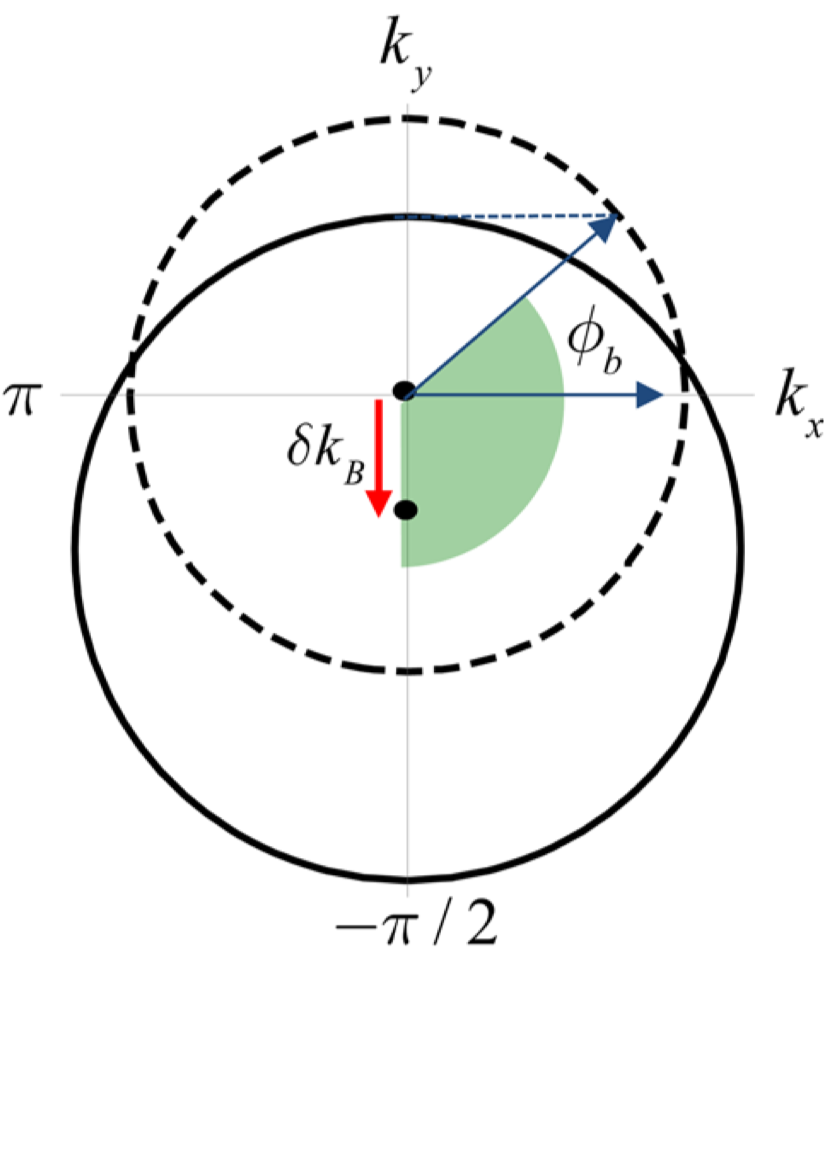
\includegraphics[width = \linewidth]{fig/Chap 2/anomalous fermi surface2.png}
            \caption{}
            \label{2fig:anomalous fermi surface2}
        \end{subfigure}
    \caption{The Fermi surfaces of Weyl cone in Fig. \ref{2fig:weyl transistor}. 
                The dashed (solid) line represents the Fermi surface in the absence (presence) of potential barrier, where Fermi energy $E_F = 82.6$ meV. 
                (a) illustrate a tilted Weyl cone where $w_y = -0.4 v_F$. 
                (b) is the non-tilted Weyl cone under the influence magnetic gauge potential.}
    \label{2fig:anomalous fermi surface}
    \end{figure}

    \begin{figure}[H]
        \centering
        \begin{subfigure}[b]{0.4\linewidth}
            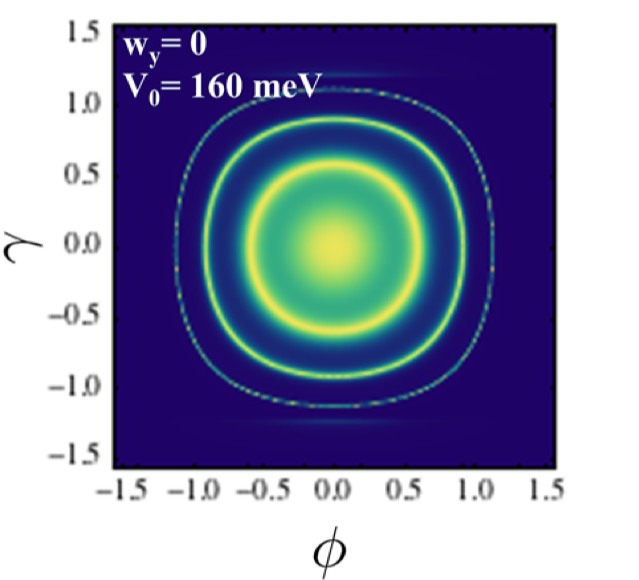
\includegraphics[width = \linewidth]{fig/Chap 2/anomalous1.png}
            \caption{}
            \label{2fig:anomalous1}
        \end{subfigure}
        \begin{subfigure}[b]{0.4\linewidth}
            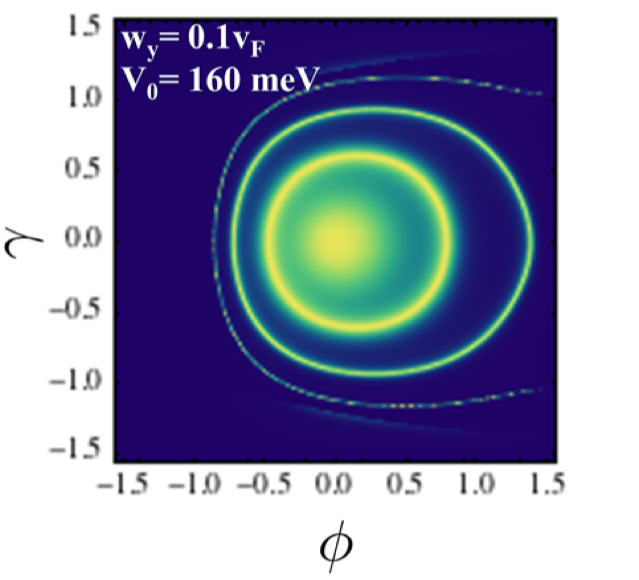
\includegraphics[width = \linewidth]{fig/Chap 2/anomalous2.png}
            \caption{}
            \label{2fig:anomalous2}
        \end{subfigure}

        \begin{subfigure}[b]{0.4\linewidth}
            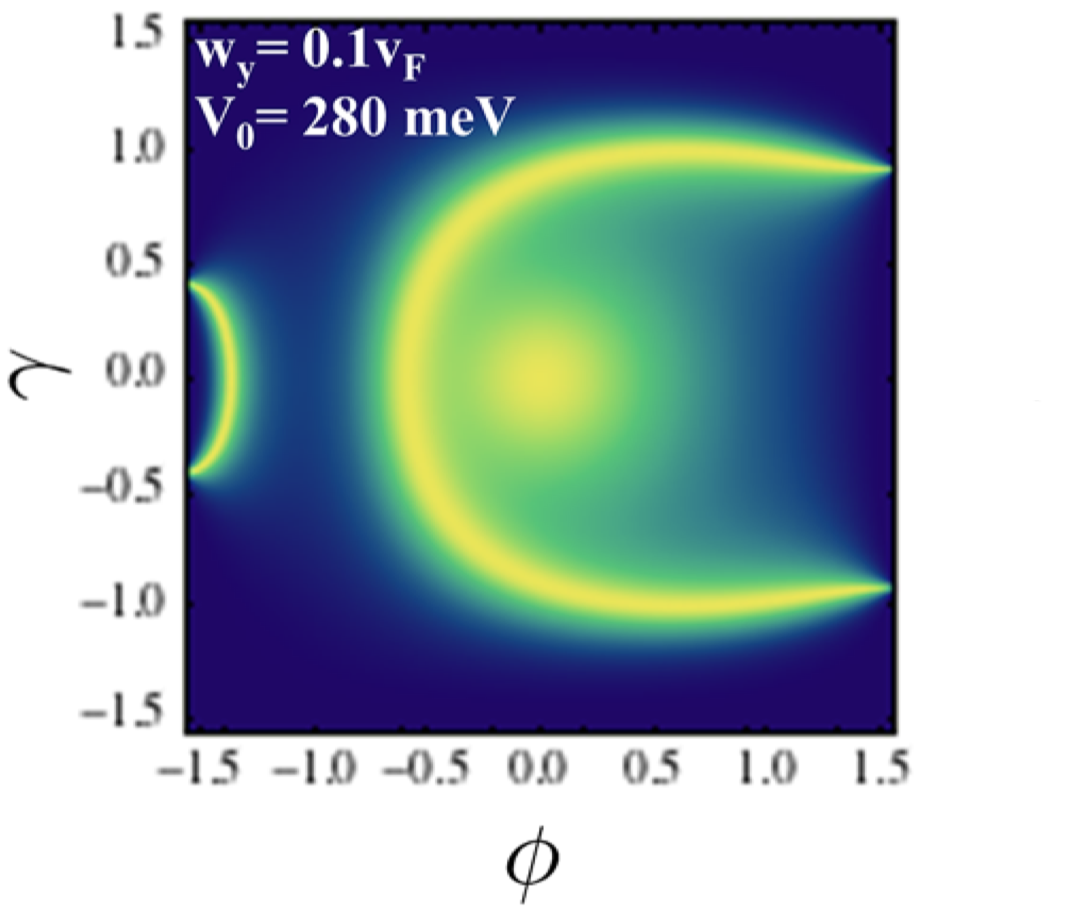
\includegraphics[width = \linewidth]{fig/Chap 2/anomalous3.png}
            \caption{}
            \label{2fig:anomalous3}
        \end{subfigure}
        \begin{subfigure}[b]{0.4\linewidth}
            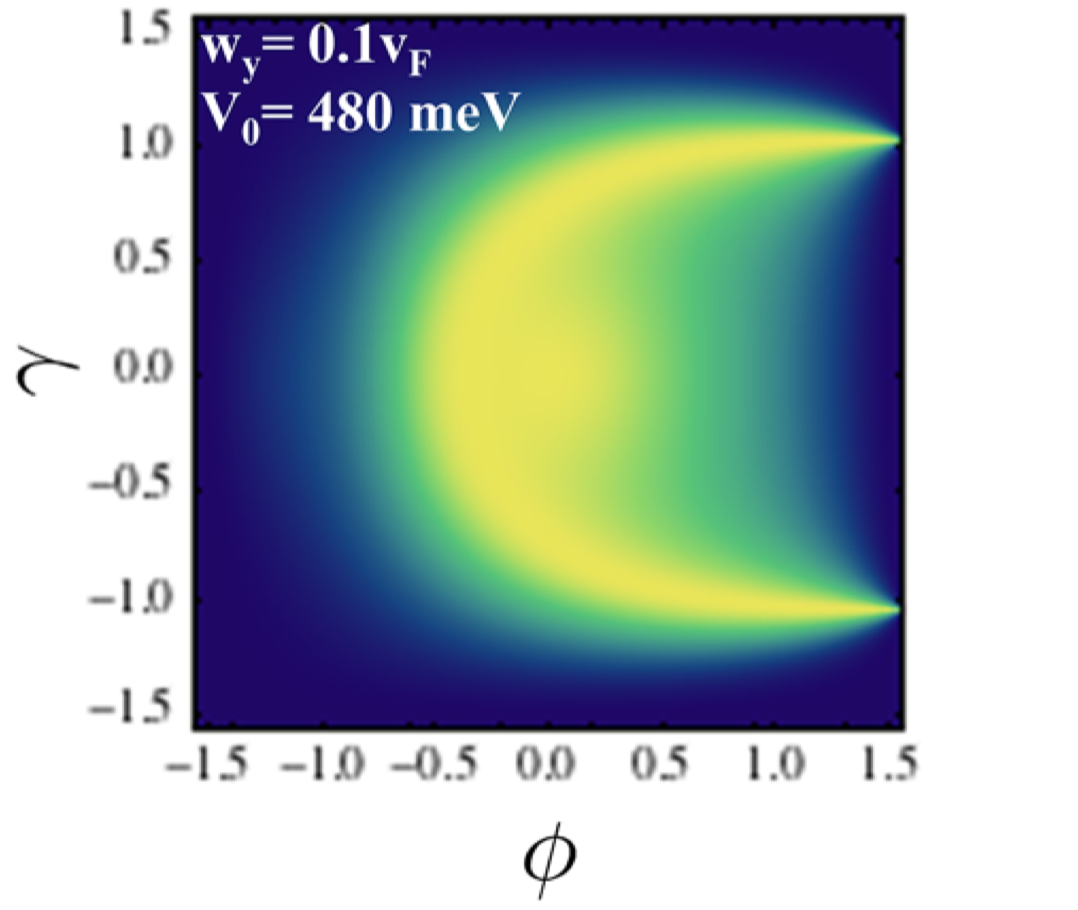
\includegraphics[width = \linewidth]{fig/Chap 2/anomalous4.png}
            \caption{}
            \label{2fig:anomalous4}
        \end{subfigure}

        \begin{subfigure}[b]{0.4\linewidth}
            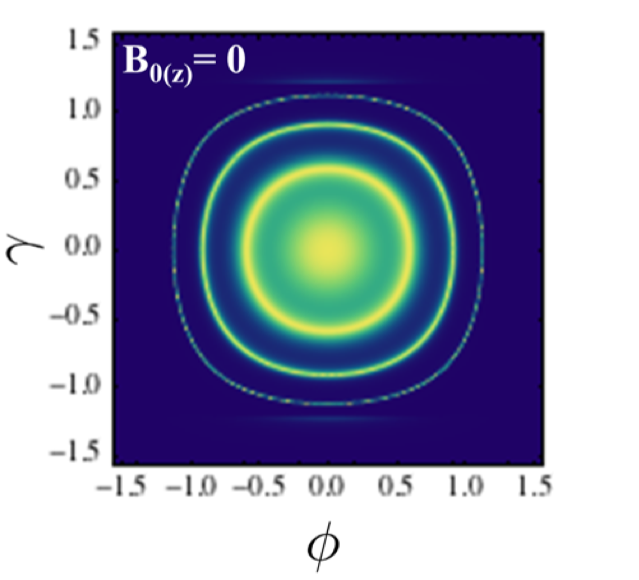
\includegraphics[width = \linewidth]{fig/Chap 2/anomalous5.png}
            \caption{}
            \label{2fig:anomalous5}
        \end{subfigure}
        \begin{subfigure}[b]{0.4\linewidth}
            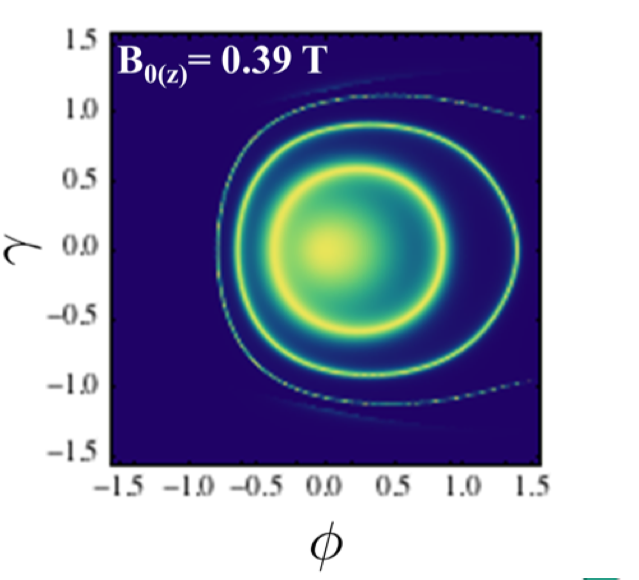
\includegraphics[width = \linewidth]{fig/Chap 2/anomalous6.png}
            \caption{}
            \label{2fig:anomalous6}
        \end{subfigure}
    \caption{The contour plot of transmission probabilities with (a) non-tilted and (b)-(d) tilted by $w_y = 0.1v_F$
                with the application of different potential barrier height in the middle region. 
                (e) and (f) show the transmission probabilities of conventional non-tilted Weyl cone
                under the influence of different magnetic field strength $B_z$. Fermi energy $E_F = 82.6$ meV, the barrier length
                $L = 100$ nm for all configurations.}
    \label{2fig:anomalous}
    \end{figure}